\chapter{Identification du sens du résultat par classification des documents}
\label{chap:sensresultat}


%Hypothèse: Les documents à une seule demande de c sont tellement nombreux que si on peut savoir si un doc n'a qu'une seule demande on peut identifier par classification le sens du résultat sur cette demande.
%
%Démonstration: 
%
%- Nb de doc à 1 dmd: si on projette la distribution des demandes dans les docs annotées, sur le corpus plus large, il est fort probable que les les doc à une demande soit majoritaires
%
%- reconnaissance des docs à 1 dmd:  par classification arbre ou ensemble-SVM à moyenne de probabilités
%
%- identification du sens du résultat: classif arbre ou ensembliste ou Gini-PLS
%
%Confiance dans les résultats (impossible du fait du faible nombre de doc - peut-être sur danais)
%
%http://www.joetsite.com/wp-content/uploads/2018/07/Vol.-72-25-18.pdf
%
%Template \verb=2011 Comparing_Mining_Algorithms_for_Predicting_the_Sev.pdf=

\section{Introduction}
\label{sec:sensresultat:motivation}
Comme le précédent, ce chapitre est relatif à l'extraction de données sur les demandes et résultats correspondants. Cependant, il est question ici d'extraire uniquement le sens du résultat d'une demande connaissant sa catégorie. Cette étude est intéressante parce que le problème devient plus simple. En se passant de la localisation précise de l'énoncé du résultat, l'extraction du sens du résultat peut être formulée comme une tâche de classification de documents. Nous modélisons la tâche comme un problème de classification binaire consistant à entrainer un algorithme à reconnaitre si la demande a été rejetée (sens = rejette) ou acceptée (sens = accepte). Cette modélisation est proposée sur une restriction du problème définie par les postulats \ref{postulat:sens:unedemande} et \ref{postulat:sens:sensbinaire} suivants.

\begin{postulat}\label{postulat:sens:unedemande}
Pour toute catégorie de demande $C$, les documents ne contenant qu'une demande de catégorie $C$ sont majoritaires. %\textcolor{red}{COMMENT SAVOIR QU'UN DOCUMENT N'A QU'UNE SEULE DEMANDE? CLASSIFICATION POSSIBLE?}
%Pour toute catégorie de demande $C$, on ne considère que les décisions dans lesquelles n'apparaît qu'une seule demande de catégorie $C$. 
\end{postulat} 
Ce postulat est légitime car les statistiques sur les données labellisées de la Figure \ref{fig:quanta:hist-repartition-docs} montre bien que dans chaque catégorie, les décisions contiennent en majorité une demande. On remarque néanmoins l'exception de la catégorie STYX (dommage-intérêt sur l'article 700 CPC), où dans la majorité des documents, on a plutôt 2 demandes. Cette exception peut se justifier par le fait que chaque partie fait généralement ce type de demande car elle porte sur le remboursement des frais de justice. Ce postulat présente cependant un inconvénient dû au fait que la majorité des demandes se trouvent dans des décisions à plus d'une demande. Il est donc possible de manquer un grand nombre de demandes. %On pourrait peut-être porter la classification à un modèle multi-label qui déterminera plusieurs sens à partir d'un seul document. Par exemple <SENS1, SENS2, SENS3> avec des valeurs prédéfinies sur les SENS 2 et 3 par exemple NO-DMD pour indiquer que la décision ne comprend pas de seconde ou de troisième demande.

\begin{postulat}\label{postulat:sens:sensbinaire}
Le sens du résultat est généralement binaire: accepte ou rejette.
\end{postulat} 
Ce postulat est justifié car le sens d'un résultat est pratiquement toujours une de ces deux valeurs (Figure \ref{stat-sensrst}). Les autres sens ne sont pas considérés car ils sont très rares.

\begin{figure}
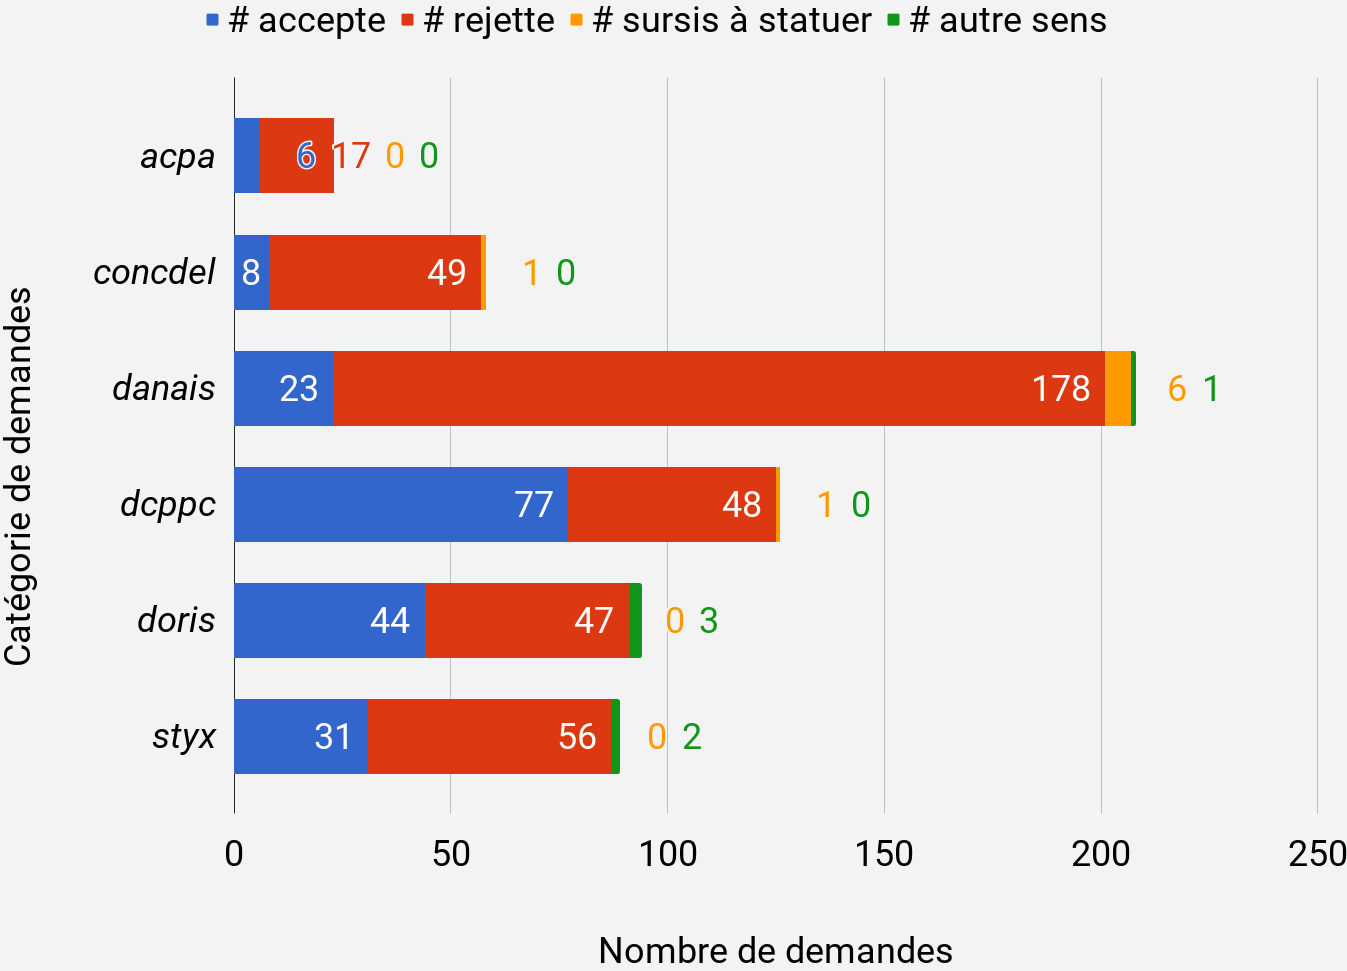
\includegraphics[width=\textwidth]{chartDistrSens.png}
\caption{Répartition des sens de résultat dans les données annotées.}\label{stat-sensrst}
\end{figure}

Cette étude porte sur l'analyse de l'impact de différents aspects techniques généralement impliqués dans la classification de texte qui consistent en générale à une combinaison de représentation des documents et d'algorithme de classification. Cette analyse permettra de savoir s'il existe une certaine configuration permettant de déterminer le sens du résultat à une demande sans nécessairement l'avoir identifiée précisément dans le document. 


\section{Classification de documents}
\label{sec:sensresultat:biblio_classif}

La classification de texte permet d'organiser des documents $x^{(k)}$ dans des groupes prédéfinis. Elle reçoit depuis longtemps beaucoup d'attentions. Deux choix techniques influencent principalement les performances: la représentation des textes et l'algorithme de classification. 

\subsection{Algorithmes traditionnels de classification de données}
Bien que la classification de documents voit se développer récemment des algorithmes propres aux textes, un grand nombre de méthodes ont été développées précédemment autour. Ces méthodes sont généralement basée sur une représentation vectorielle des textes et délimitent une frontière entre les classes dans un espace multidimensionnel. 
%NB et SVM : https://www.dropbox.com/home/Documents/to-read/term-weight?preview=Best+Terms+An+Efficient+Feature+Selection+Algorithm+for+Text+Categorization.pdf
% C4.5, k-means, svm, apriori algo, em algo, page rank, ada boost, knn, NB, CART: http://www.cs.umd.edu/~samir/498/10Algorithms-08.pdf

\subsubsection{Le Bayésien naïf (NB)}
\paragraph{Principe}:
%http://stackoverflow.com/questions/10059594/a-simple-explanation-of-naive-bayes-classification#20556654
%https://webdocs.cs.ualberta.ca/~greiner/R/PAPERS/ExplainNB.pdf
Les classifieurs naïfs bayésiens \citep{duda1973patternclass} sont des modèles à densité qui estiment la probabilité qu'un texte appartienne à une classe à partir du théorème de Bayes \citep{raschka2014naivebayes}:
\begin{equation}
\text{probabilité a posteriori} = \frac{\text{probabilité conditionnelle} \cdot \text{probabilité a priori}}{\text{évidence}}
\end{equation}

La probabilité a posteriori peut être interprétée dans le cadre de la classification des décisions dans la classe DIPA en "Quelle est la probabilité qu'une décision $t_i$ contienne une demande de type $c_j$ étant donné que $t$ contient les termes $\lbrace w_1, ..., w_K \rbrace$ ?". La réponse à cette question se formalise comme suit:

\[\p(c_j \vert t_i) = \frac{\p(t_i \vert c_j)\p(c_j)}{\p(t_i)}\]
ou plus simplement  $\p(c_j \vert t_i) = \p(c_j)\p(t_i \vert c_j)$ car $\p(t_i)$ ne change pas en fonction de la catégorie et peut donc être ignorée \citep{rish2001nb_study}.
L'appélation "\textit{naïf}" est dûe à l'hypothèse d'\textbf{indépendance mutuelle entre les caractéristiques} des données. Une hypothèse %irréaliste 
forte dont la violation, par les données réelles, n'empêche pourtant pas les NB de bien fonctionner \citep{rish2001nb_study}. 

\begin{hypothese}[indépendance mutuelle des caractéristiques] [ Un modèle naïf bayésien étant de type génératif], la position de chaque mot dans le texte est générée indépendament de tout autre mot étant connue la catégorie du texte. \label{hypo_imc}
\end{hypothese}
% je l'aurais fait avec les demandes directement à voir...on voit bien dans ce cas que l'hypothèse d'indep est trop forte.

\noindent L'hypothèse \ref{hypo_imc} implique, pour des catégories de demande indépendantes,
\[
\mathbb{P}(d_{i1}, \dots, d_{iK}\vert c_j) = \prod_{k=1}^K \p(d_{ik} \vert c_j).
\]
Ainsi,
\begin{equation}\notag
\mathbb{P}(c_j\vert d_{i1}, \dots, d_{iK}) = \frac{\p(c_j)\p(d_{i1}, \dots, d_{iK} \vert c_j)}{\p(d_{i1}, \dots, d_{iK})} = \frac{\p(c_j)\prod_{k=1}^K \p(d_{ik} \vert c_j)}{\p(d_{i1}, \dots, d_{iK})}.
\end{equation}
La fonction score issue de ce classifieur bayésien est construite en maximisant la probabilité $\mathbb{P}(c_j\vert d_{i1}, \dots, d_{iK})$. Il n'est donc pas nécessaire de connaître ni d'estimer la probabilité jointe $\p(d_{i1}, \dots, d_{iK})$.

\paragraph{Estimation des paramètres}: 
% là tu introduits les w_i. Il faudrait donc compléter la section 2.1 stp. 

%quand tu parles de paramètres tu penses à quoi exactement ? pour moi ce serait ceux de la fonction score...

Grâce à l'hypothèse \ref{hypo_imc}, la probabilité conditionnelle ($\p(t_i \vert c_j$)) peut-être réécrite:
\[\p(t_i \vert c_j) = \p(w_1 \vert c_j)\cdot \p(w_2 \vert c_j) \cdot ... \cdot \p(w_d \vert c_j) = \prod\limits_{k = 1}^d \p(w_k \vert c_j)\]
pour une représentation vectorielle des textes dans un espace de dimension $d$.
Les paramètres du modèle peuvent donc être estimés à partir d'un jeu d'exemples d'entrainement. Plus précisément, $\forall k \in \lbrace 1, 2, ..., d \rbrace: \p(w_k \vert c_j) = \frac{N_{wc_j}}{N_{c_j}}$ et $\p(c_j) = \frac{N_c}{N}$.

Actuellement, les algorithmes NBSVM et FastText sont les plus populaires pour la classification de documents et ont les performances pour l'analyse de sentiment sont très bonnes. L'ensemble des labels / classes est noté $C$.

\textcolor{red}{VARIANTE}

\subsubsection{Machine à vecteurs de support (SVM)}
Le SVM \citep{vapnik1995statlearning} est un algorithme de classification binaire, qui construit, lors de la phase d'entrainement un hyperplan séparant les points, représentants les exemples d'entrainement, dans un espace à grande dimension, suivant leur classe (Figure \ref{fig:sensresultat:svm}\footnote{\url{http://www.clrc.rhul.ac.uk/svm.html}}). L'hyperplan est la surface situé entre les droites formées par les points les plus proches des deux classes. La classification d'un nouvel objet consiste à projeter son vecteur de caractéristiques dans cet espace, et le label qui lui est prédit est celui associé à la classe du coté où il se trouve. La projection d'une entrée $x$ dans le nouvel espace, est réalisée par une fonction non-linéaire appelé noyau.

\textcolor{red}{optimisation de la fonction objectif pour l'entrainement, + calcul des hyperparamètres}

\begin{figure}[!htb]
	\centering
	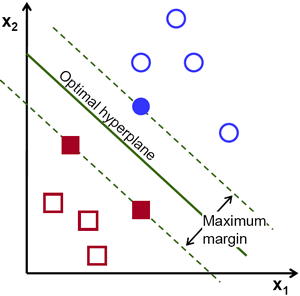
\includegraphics[scale=2]{svm.png}
	\caption{Illustration de l'hyperplan d'un SVM.}\label{fig:sensresultat:svm}
\end{figure}

\subsubsection{$k$-plus-proches-voisins (kNN)}
L'algorithme $k$-plus-proches-voisins est un algorithme très simple qui consiste à affecter à un nouvel objet la classe majoritaire $y'$ parmi ceux des $k$ points d'exemples d'entrainement $\lbrace (x_i,y_i) \rbrace_{1:k}$, les plus proches du point $x'$ de cet objet selon la métrique $d$ choisie. Ainsi, trois éléments clés influencent l'efficacité de la classification:
\begin{enumerate}
	\item les données d'entrainement dont le nombre s'il est très grand peut rendre chère le processus de classification, car la distance du nouvel objet à chaque point annoté, est calculée;
	\item le nombre de voisins (c'est-à-dire la valeur de $k$) qui ne doit être ni très petit (sensibilité aux bruits / \textit{outliers}), ni très grand (risque d'avoir dans le voisinage beaucoup de points d'une autre classe). La sensibilité au nombre de voisins peut être atténuée en pondérant les points par leur distance à l'objet à classer. La stratégie de choix de la classe du nouvel objet est ainsi appelé \og vote pondéré par la distance \fg{}: \[y' = \argmax\limits_c \sum\lim\limits_{(x_i,y_i)} \frac{1}{d(x', x_i)^2} \times I(c = y_i)\] où $I(c=y_i) = \left\lbrace \begin{array}{ll}
	1 & \text{si }c \text{ est égal à } y_i \\
	0 & \text{sinon}
	\end{array} \right.$
	\item la métrique de calcul de distance qui doit être adéquate pour le type de donnée et la tâche (par exemple, la distance cosinus est préférable à la distance euclidienne pour la classification de documents, la deuxième métrique se dégradant lorsque le nombre d'attributs augmente).
\end{enumerate}


\subsubsection{Arbre de décision}
Un arbre de décision est structure arborescente utilisée en fouille de données pour associer un label prédéfini à des objets (classification), ou prédire la valeur d'une variable continue (régression). Il comprend en des noeuds internes qui correspondent chacun à un test sur la valeur d'un attribut (test uni-varié), des arêtes correspondant à une sortie du test, et enfin des feuilles ou noeuds terminaux qui correspondent chacune à une prédiction. L'algorithme de classification d'un nouvel objet avec l'arbre de décision est très simple (Algorithme \ref{algo:sensresultat:classifywithtree}).

\begin{algorithm}[H] \small
	\KwData{Objet $x$, Arbre $A$}
	\KwResult{label}
	$n := racine(A)$ \; 
	\While{$n$ n'est pas une feuille}{
		Effectuer sur $x$ le test associé à $n$\;
		$n :=$ noeud fils de $n$ correspondant au résultat du test \;
	}
	\Return le label associé à la feuille $n$\;
	\caption{Classification d'un objet à l'aide d'un arbre de décision} \label{algo:sensresultat:classifywithtree}
\end{algorithm}

La construction de l'arbre, c'est-à-dire l'apprentissage, consiste à générer une hiérarchie de tests, aussi courte que possible, qui divise successivement l'ensemble $S$ d'exemples d'apprentissage en sous-ensembles disjoints de plus en plus pures\footnote{homogénéité des labels}. %, tels que des sous-groupes de cas appartenant à la même classe soient rapidement détectés. 
L'arbre est construite de la racine aux feuilles en divisant les données d'entrainement $S_{t}$ à chaque étape ($t$) de sorte à minimiser le degré d'impureté des sous-ensemble d'exemples  $S_{t_i}$ dans les nœuds fils ($t_i$). Les divers algorithmes de construction diffèrent par le critère (ou la métrique) de séparation. Un critère de coupe est généralement défini à partir d'une métrique d'impureté comme par exemple:
\begin{itemize}
	\item l'entropie de la distribution des classes dans $S_t$: \[h_C(S_t) = - \sum\limits_{c \in C} \left[p(c \vert S_t) \log_2 p(c \vert S_t)\right];\]
	\item l'indice de Gini mesurant la divergence entre les distributions de probabilité des valeurs de la variable prédite: \[g_C(S_t) = 1 - \sum\limits_{c \in C} \left[p(c \vert S_t)\right]^2;\]
	\item l'erreur de classification définie par : \[e_C(S_t) = 1 - \max\limits_{c \in C} \left[p(c \vert S_t)\right]\]. 
\end{itemize}
Pour ces métriques, $p(c \vert S_t)$ représente la proportion d'exemples du nœud $t$ appartenant à $c$, et $S_t$ représente . Parmi les critères de séparation les plus populaires associés à ces critères, on retrouve: 

\begin{itemize}
	\item le gain d'information apporté par le test $t$ portant sur l'attribut $a$ (qui divise $S_t$ en des sous-ensembles $S_{t_i}$) utilisant l'entropie comme métrique d'impureté, et est définie par la différence entre l'entropie de $t$ et l'entropie moyenne des fils de $t$:  \[ig(S_t, a) = h_C(S_t) - i(S_t, t, a) =  h_C(S_t) - \sum\limits_{S_{t_i}} \frac{\vert S_{t_i} \vert}{\vert S_{t} \vert} \cdot h_C(S_{t_i});\]
	\item le rapport des gains, qui corrige le gain d'information, biaisé en faveur des tests ayant un grand nombre d'alternatives (sorties du nœud), en prenant en compte l'information intrinsèque $h_t(S_t)$ de la séparation de $S_t$ suivant le test $t$ en sous-ensembles $S_{t_i}$: \[gr(S_t, t, a) = \frac{ig(S_t, t, a)}{h_t(S_t)} \text{ avec } h_t(S_t) = \sum\limits_i \frac{\vert S_{t_i}\vert}{\vert S_t \vert} \log_2 \left(\frac{\vert S_{t_i}\vert}{\vert S_t \vert}\right)\]
	\item le critère binaire de "doublage" (\textit{twoing criteria}) qui ne s'emploie dans les arbres binaires : \[tc(t) = \frac{P(S_{t_R} \vert S_t)P(S_{t_L} \vert S_t)}{4} \left[\sum\limits_{c \in C} \vert p(c \vert t_L) - p(c \vert t_R)\vert\right]^2\] où  $P(S_{t_R} \vert S_t)$ et $P(S_{t_L} \vert S_t)$ sont les proportions de $S_t$ qui vont respectivement dans les fils $t_R$ et $t_L$ après séparation suivant le test $t$.
\end{itemize}

Les variables nominales peuvent être divisées soit en utilisant autant de partitions que de valeurs distinctes (partition multiple), soit uniquement en des partitions binaires suivant des tests booléens (partition binaire) nécessitant de rechercher la division optimale. Les variables numériques sont divisées quant à elles soit suivant par discrétisation de leur domaine les transformant en variables catégoriques ordinales, soit en recherchant la meilleure division binaire parmi  toutes les séparations possibles. 

La construction de l'arbre étant une division récursive de noeud qui peut continuer tant qu'il est possible d'améliorer la pureté des noeuds, ce qui peut engendrer un arbre très grand résultant en un sur-apprentissage\footnote{Un modèle trop précis a un très faible taux d'erreur sur les données d'entrainement (erreur d'apprentissage) mais un fort taux d'erreur pour les données de test (erreur de test).}. Pour s'arrêter plus tôt ("pré-élagage"), plusieurs conditions sont possibles comme par exemple, l'atteinte par la taille des données ($\vert S_t \vert$) d'un seuil minimum, ou l'atteinte par l'arbre d'une profondeur maximale, ou l'amélioration du critère de division est très faible, etc. Le post-élagage est appliqué après construction de l'arbre toujours dans le but de minimiser le sur-apprentissage.

Les algorithmes de construction d'arbres diffèrent ainsi par leur critère de séparation, leur stratégie d'élagage, et leur capacité à gérer les types d'attributs, les valeurs manquantes et extrêmes. \citet{singh2014id3cartc45} comparent ainsi les deux algorithmes CART et C4.5 que nous avons utilisés (Tableau ).

\begin{table}
	\begin{tabular}{|l|p{1.5cm}|p{1.5cm}|p{1.5cm}|p{1.5cm}|p{1.5cm}|p{1.5cm}|}
		\hline
		& Critère de séparation & Variables numériques & Valeurs manquantes & Stratégie d'élagage & Détection de valeurs extrêmes & Implémentations \\ \hline
CART   & critère de "doublage" & supportées & supportées & élagage à coût complexe & supportées  & Sckit-learn \\ \hline
C4.5 & rapport des gains & supportées & supportées & élagage basé sur l'erreur & susceptible & J48 (Weka) \\ \hline
	\end{tabular}
\end{table}

%Les arbres de décisions sont des structures graphiques qui organisent sur un arbre les valeurs des caractéristiques dans des n\oe{}uds parents et les sorties au niveau des feuilles. Le principe de prédiction à l'aide des arbres consiste à construire le chemin allant de la racine à une feuille suivant les valeurs des caractéristiques présentées en entrée. Deux algorithmes de construction d'arbres de décision sont très populaires; il s'agit du CART (\textit{Classification and Regression Trees}), implémenté dans la librairie Scikit-Learn [?], et C4.5, implémenté dans la librairie Weka sous le nom de J48.
%
%\textcolor{red}{Expliquer le fonctionnement général d'un arbre de décision à partir d'un exemple illustré (\url{https://towardsdatascience.com/what-is-the-c4-5-algorithm-and-how-does-it-work-2b971a9e7db0})}
%
%Un CART est représenté par un arbre binaire dont chaque n\oe{}ud est défini par une condition sur la valeur d'une variable d'entrée, et comme les deux n\oe{}uds fils de correspondent respectivement aux deux valeurs VRAI ou FAUX de la condition. Chaque feuille de  l'arbre correspond à une prédiction pour la variable de sortie. Pour prédire la valeur de sortie pour un nouvel objet présenté en entrée, il suffit de traverser l'arbre de la racine à une feuille en suivant le chemin correspondant aux caractéristiques de cet objet.
%
%L'entrainement d'un arbre consiste à le construire, i.e. à trouver les conditions adéquates sur les variables descriptives, ainsi que leur enchainement adéquat. Il existent plusieurs algorithmes de construction d'arbre qui minimise l'erreur sur la base d'entrainement. Par exemple, le "découpage glouton" (\textit{Greedy Splitting}) consiste à construire successivement les noeuds de l'arbre, en sélectionnant la variable et la valeur de coupe optimale pour discriminer les classes au niveau du noeud courant. Pour la classification binaire, la métrique d'erreur à minimiser implique l'indice de Gini (indice de pureté du sous-arbre d'intérêt): \[G = \sum(p_k * (1-p_k)) = 2p_1p_2\] où $p_k$ est la proportion d'élément de la classe $k$ dans le sous-arbre d'intérêt.
%Cet indice est pondéré par le nombre d'instances d'entrainement dans le noeud parent: \[G = \frac{n_1}{n}(2p_{11}p_{21}) + \frac{n_2}{n}(2p_{12}p_{22}) \], $n_j$ étant le nombre d'instance dans le groupe $j$, et $p_{ij}$ est la proportion d'instances de la classe $i$ dans le groupe $j$.
%Une condition d'arrêt de construction de l'arbre généralement utilisée est l'infériorité du nombre d'instances du noeud par rapport à un seuil minimum défini en deçà duquel aucun découpage n'est permis. Le noeud respectant la  condition d'arrêt est une feuille et la classe qui lui est assignée est la classe majoritaire à ce noeud (\textcolor{red}{àvérifier?}).
%
%L'arbre ayant été construit successivement et localement, pour optimiser son efficacité (éviter le sur-apprentissage), il faut élaguer les branches d'impact négatif sur la qualité des résultats. La méthode utilisée consiste généralement à évaluer successivement l'effet de suppression des feuilles de l'arbres, et à éliminer celles cet effet est positif sur l'erreur obtenu sur une base de validation (\textcolor{red}{le tuto parle d'ens de test \textit{hold-out}}). 
%
%\textcolor{red}{Quelles techniniques utilise sklearn??}
%
%
%Quant au C4.5, il s'agit d'un algorithme de classification produisant un arbre de décision basée sur la théorie de l'information. En effet, la meilleure variable pour le découpage à un noeud est celle qui porte le gain d'information normalisé le plus important.
 
\subsubsection{Analyses discriminantes linéaires et quadratiques}

L'analyse discriminante comprend l'ensemble des méthodes déterminant les combinaisons linéaires de variables qui permettent de séparer le mieux possible $K$ catégories ou variables qualitatives. Les analyses linéaires et quadratiques sont des méthodes probabilistes basées sur la probabilité conditionnelle d'appartenance d'un objet $X$ à une classe $y_k$: \[P(Y=y_k \vert X) = \frac{P(Y=y_k) P(X \vert Y=y_k)}{P(X)} = \frac{P(Y=y_k) P(X \vert Y=y_k)}{\sum\limits_{j = 1}^K P(Y=y_j) P(X \vert Y=y_j)}\].
La classe de $X$ est donc $y_{k*} = \argmax_k P(Y=y_k \vert X) = P(Y=y_k) P(X \vert Y=y_k)$ car le dénominateur est le même pour toutes les classes. Dans cette expression, $P(Y=y_k)$ est la proportion d'exemples de classes $y_k$ dans l'ensemble des données d'apprentissage. Il ne reste donc qu'à déterminer $P(X \vert Y=y_k)$, pour trouver $y$. Deux hypothèses simplifient les calculs:
\begin{enumerate}
	\item l'hypothèse de normalité statuant que la probabilité conditionnelle $P(X \vert Y)$ suit une loi normale multidimensionnelle: \[P(X \vert Y = y_k) = \frac{1}{\sqrt{2\pi det(\sum_k)}}e^{-\frac{1}{2}(X - \mu_k)\sum_k^{-1}(X - \mu_k)'} \] $\mu_k$ étant le centre de gravité conditionnelle, et $\sum_k$ la matrice de variance covariance conditionnelle;
	\item l'hypothèse d'homoscédasticité statuant que les matrices de variance co-variance conditionnelles sont identiques i.e.: \[\forall j,k \in \lbrace 1,...,K \rbrace, \sum_j = \sum_k = \sum.\]
\end{enumerate}

L'analyse discriminante linéaire (LDA) est définie par une simplification de $P(X \vert y_k)$ sous ces deux hypothèses. En effet, grâce à la proportionnalité de la probabilité conditionnelle à :$\ln\left[P(X \vert y_k)\right] \propto -\frac{1}{2}( X - \mu_k )\sum^{-1}(X - \mu_k )'$, on déduit une fonction discriminante (ou de classement) linéaire proportionnelle à $P(y_k \vert X)$: \[d(y_k, X) = \ln\left[P(Y = y_k)\right] + \mu_k \sum^{-1}X' - \frac{1}{2}\mu_k\sum^{-1}\mu_k'.\] Ainsi $y_{k*} = \argmax_{k \in \lbrace 1,...,K \rbrace} d(y_k, X)$.

L'analyse discriminante quadratique (QDA) considère l'hétéroscédasticité (i.e. $\exists k \neq j, \sum_k \neq \sum_j$), et donc ne s'appuie que sur la 1e hypothèse (multinormalité). Dans ce cas, on obtient une règle quadratique de classification $k* = \argmax_{k \in \lbrace 1,...,K \rbrace} Q_k(X)$ où:
\[Q_k(X) = (x - \mu_k)'\sum_k^{-1}(x - \mu_k) - 2 \ln(\pi_k) + \ln(det(\sum_k))\] est la fonction quadratique de classement de la classe $k$.

%\subsubsection{Modèles ensemblistes}


\subsection{Algorithmes dédiés aux textes}

\subsubsection{NBSVM}

Le NBSVM \citep{wang2012nbsvm} est un classifieur binaire (deux labels $\lbrace -1; 1 \rbrace$) dont le principe consiste à transformer les poids $f^{(k)}$ caractéristiques $V$ des textes $x^{(k)}$, réduites à leur simple présence $\widehat{f}^{(k)}$ en réalisant leur produit élément à élément ($\overset{\sim}{f}^{(k)} = {r} \circ \widehat{f}^{(k)}$) avec le vecteur de poids $r$ du classifieurs bayésien multinomial (calculé avec le vecteur présence de caractéristique):
$r = \log \left( \frac{p/\vert\vert p \vert\vert_1}{q / \vert\vert q \vert\vert_1}\right)
\text{ avec } p=\alpha + \sum\limits_{k:y^{(k)}=1}{f}^{(k)}$, $q=\alpha + \sum\limits_{k:y^{(k)}=-1}{f}^{(k)}$. L'ensemble des caractéristiques $V$ est constitué de n-grammes de mots. Le nouveau vecteur issu de ce produit représente le texte ($x^{(k)} = \overset{\sim}{f}^{(k)}$) en entrée d'un SVM classique. La classe de $x^{(k)}$ est prédite par : $y^{(k)} = sign(\mathbf{w}^Tx^{(k)} + b)$, $\mathbf{w}$ et $b$ étant appris lors de l'entraînement du SVM. Une interpolation  entre le bayésien multinomial et le SVM est nécessaire pour assurer la robustesse du NBSVM et des performances excellentes pour toute tâche de classification de documents; les poids $\mathbf{w}$ sont réajustés par le model $\mathbf{w'} = (1 - \beta) \overline{w} + \beta \mathbf{w}$, où $\overline{w} = \vert\vert \mathbf{w}\vert\vert_1 / \vert V \vert$ et $\beta \in \left[0; 1] \right.$. 
  
  
  \subsubsection{FastText}
  
 FastText \citep{grave2017fasttextcls}, quant à lui, est un modèle de réseau de neurones dont l'architecture est semblable à celle de la variante CBOW de la méthode de plongement sémantique Word2Vec dans laquelle le mot du milieu a été remplacé par le label de la classe du texte et au dessus de laquelle la fonction softmax $f(z) = \left[ \frac{e^{z_j}}{\sum\limits_{k=1}^K e^{z_k}} \right]_{\forall j \in \lbrace 1, ..., K \rbrace} $ est rajoutée pour réaliser la classification à partir de la représentation distribuée du texte. La phase d''entraînement consiste à minimiser la fonction objectif $-\frac{1}{N}y_n \cdot \sum\limits_{n=1}^N y_n \cdot \log{f(B\cdot A\cdot x_n)}$ qui estime la distribution de probabilité des classes.

Ces deux méthodes intègrent leur propre représentation de document, contrairement aux algorithmes opérant sur dans des espaces vectorielles aux axes et poids paramétrables à volonté comme le SVM. Il existe un très grand nombre de schémas de représentations des documents.

NBSVM et Fastext ont démontré une bonne robustesse et et des performances excellentes dans le cas de divers tâches de classification: courtes expressions, longs documents, thème, classification subjective (genre), classification de sentiment (positif, neutre, négatif), ... Mais nous voulons déjà savoir comment les algorithmes populaires se comportent sur notre tâche d'identification de la polarité du résultat d'une demande pour une catégorie bien définie. La particularité ici est que la tâche porte sur une demande en particulier parmi les nombreuses que compte le document, des données en faible nombre annotés (23 à 189 documents), une annotation en général déséquilibrée entre les classes (risque d'ignorer une classe très faiblement représenté dans le jeu d'entrainement, par exemple 21 "accepte" contre 166 "rejette").

\subsection{Discussion: Techniques d'amélioration de la précision}
Livre Data mining 

\section{La Regression PLS et ses extensions}
\label{sec:sensresultat:pls}
\textcolor{red}{Justification: Pourquoi le PLS?:}
%https://link.springer.com/content/pdf/10.1007\%2FBF02174528.pdf, 
%https://www.stat4decision.com/fr/regression-pls/
La regression PLS est une méthode de regression avec laquelle l'on tente d'expliquer une ou plusieurs variables Y (dite dépendantes) par des variables $X=x_1,x_2,...,x_p$ (dites explicatives). Elle consiste principalement à transformer les variables explicatives en un nombre réduit de composantes principales orthogonales $t_1, t_2, ..., t_h$. Les composantes $t_h$ sont construites étapes par étapes en applicant l'algorithme du PLS de façon récurrente sur les données mal prédites (résidus). Plus précisément, à chaque itération $h$, la composante $t_h$ est calculée par la formule $t_h = w_{h1} x_1 + \cdots + w_{hj} x_j + \cdots + w_{hp} x_p$. 

Malgré quelques faiblesses comme celles liées au choix du nombre de composantes, à la complexité des sorties et la linéarité du modèle, la regression PLS présente quelques atouts qui ont notamment de l'intérêt dans notre cas de figure. Par exemple, le PLS gère assez bien la forte disproportion entre le nombre de variables explicatives et le nombre d'observations, lorsque ce dernier est faible comme on peut l'observer dans nos données (faible quantité de données d'apprentissage). Nous avons aussi la prise en compte de la multicolinéarité qui peut exister entre les variables explicatives, notamment quand celles-ci sont associées aux mots/termes souvent cooccurrents de nos documents.

Il est intéressant de noter la floraison d'extensions proposées pour répondre aux différentes limites du PLS. Notamment, nous pouvons citer la "\textit{sparse}" PLS introduite pour palier à la "\textit{sparsité}" et la colinéarité des variables explicatives [?], la PLS non-linéaire proposée pour les cas de données non-linéairement séparables [?], ou encore la PLS discriminante combinant la régression PLS et l'analyse discriminante [?]. Nos nous sommes intéressés à deux extensions particulières: la régression Gini-PLS \citep{mussard2018ginipls} dont l'intérêt est de réduire la sensibilité aux valeurs aberrantes des variables, et la regression Logit-PLS \citep{tenenhaus2005logitpls}  combinant la regression logistique et la PLS.
\subsection{Gini-PLS}
Cette méthode élimine la sensibilité du PLS aux valeurs extrêmes en remplaçant la covariance $cov(x_j, y)$ par la covariance de Gini $cog(y; x_j) := cov(y; R(x_j))$ pour l'estimation des résidus $u_{(h)j}$ et des poids $w_{hj}$ \citep{mussard2018ginipls}.


\subsection{Logit-PLS}
Dans cette approche, $\forall j > 1$, les $w_{hj} $ sont les coefficients de la régression logistique de $y$ sur les composantes $t_1, ..., t_{h-1}, u_{(h-1)j}$ \cite{tenenhaus2005logitpls}.

\subsection{Gini-Logit-PLS}
Cette approche combine la covariance Gini pour $u_{(h)j}$ et le coefficient Logit pour les $w_{hj}$.


\section{Méthode}
Nous raisonnons toujours suivant une seule catégorie $c$. Notre solution est une chaîne à 2 étapes de classification: un filtre des décisions à une demande de la catégorie $c$ et un identificateur de la polarité du résultat. Le premier classifieur discrimine les document entre 2 classes: \og une demande \fg{} et \og plusieurs demandes \fg{}.

\section{Expérimentations et résultats}
\label{sec:sensresultat:experimentations}
Nous discutons ici les performances de divers algorithmes populaires et l'impact de la quantité et du déséquilibre des données, de la restriction à des passages en particulier, ainsi que leur capacité à faire abstraction des autres demandes du document. 

\subsection{Protocole d'évaluation}
Deux métriques d'évaluation sont utilisées: la précision et la F1-mesure. Pour tenir compte du déséquilibre entre les classes, la moyenne macro est préférée (agrégation de la contribution individuelle de chaque classe: $F1_{moyenne} = \frac{1}{2}(F1({accepte}) + F1({rejette}))$).

Les données utilisées sont les mêmes que celles du chapitre précédent. Nous avons seulement fait une restriction sur les documents n'ayant qu'une seule demande annotée pour la catégorie considérée. Le déséquilibre entre les classes est illustrée par la figure \ref{fig:sensresultat:stat-1dmd}. En effet, la demande est plus souvent rejetée qu'acceptée pour les catégorie ACPA, CONCDEL, DANAIS et STYX. Le contraire est observé pour DCPPC et DORIS.
\begin{figure}[htb]
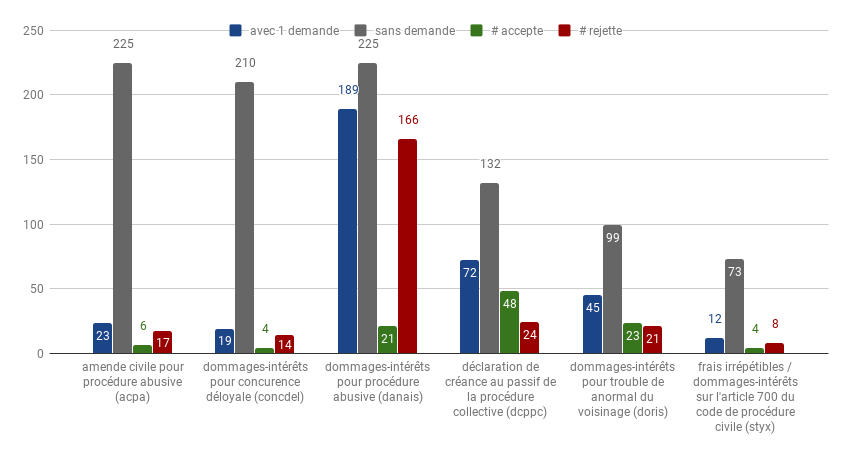
\includegraphics[width=\textwidth]{chartDataset1dmd.png}
\caption{Répartition des documents à une demande de la catégorie considérée.}\label{fig:sensresultat:stat-1dmd}
\end{figure}

\subsection{Classification de l'ensemble du document}

En représentant l'ensemble du document à l'aide de diverses représentations vectorielles, les algorithmes sont comparés avec les représentations qui leurs sont optimales. On remarque d'après les résultats du Tableau \ref{tab:sensrst:global}, les arbres sont en moyenne meilleurs sur l'ensemble des catégories même si en moyenne la F1-mesure moyenne est limité à 0.668. Les résultats des extensions du PLS ne sont pas très éloignée de ceux des arbres avec des différences de F1 à moins de 0.1 (si on choisi le bon schéma de "vectorisation").

\begin{table}[!htb]	
	\tiny
	
	\textcolor{red}{ajouter les F1 ou erreur de rejette et de accepte}
	
	\begin{tabular}{|l|l|l|l|l|l|l|l|l|l|}
		\hline
		\textbf{Vecteur} & \textbf{algorithme} & \textbf{F1} & \textbf{min} & \textbf{Cat. min} & \textbf{max} & \textbf{Cat. max} & \textbf{F1 - 1erF1} & \textbf{max - min} & \textbf{rang} \\ \hline
		GSS*TF           & Arbre               & 0.668       & 0.5          & doris             & 0.92         & dcppc             & 0                   & 0.42               & 1             \\ \hline
		AVG-G*TF         & LogitPLS            & 0.648       & 0.518        & danais            & 0.781        & dcppc             & 0.02                & 0.263              & 13            \\ \hline
		AVG-G*TF         & StandardPLS         & 0.636       & 0.49         & danais            & 0.836        & dcppc             & 0.032               & 0.346              & 24            \\ \hline
		DELTADF*TF       & GiniPLS             & 0.586       & 0.411        & danais            & 0.837        & dcppc             & 0.082               & 0.426              & 169           \\ \hline
		DELTADF*TF       & GiniLogitPLS        & 0.578       & 0.225        & styx              & 0.772        & dcppc             & 0.09                & 0.547              & 220           \\ \hline
		-                & NBSVM               & 0.494       & 0.4          & styx              & 0.834        & dcppc             & 0.174               & 0.434              &               \\ \hline
		-                & FastText            & 0.412       & 0.343        & doris             & 0.47         & danais            & 0.256               & 0.127              &               \\ \hline
	\end{tabular}
\caption{Comparaison des algorithmes sur une représentation globale des documents pour la détection du sens du résultat.}\label{tab:sensrst:global}
\end{table}

 Les scores F1 moyens des algorithmes  NBSVM et FastText n'excédent en général pas 0.5 malgré qu'ils soient spécialement conçus pour les textes.  Soit ils sont très sensibles au déséquilibre des données entre les catégories (plus de rejets que d'acceptations), soit il est plus difficile de détecter l'acceptation des demandes. En effet, ces algorithmes classent tous les données de test avec le label (sens) majoritaire i.e. le rejet, et par conséquence, ils ne détectent peu ou pas d'acceptation de demande. Le cas des catégories DORIS et DCPPC pour le NBSVM (F1-macro moyen = 0.834) tend à démontrer la forte sensibilité aux cas négatifs de ces algorithmes puisque même avec presque autant de labels "accepte" que "rejette", la F1-mesure de rejette est toujours supérieure à celle de "accepte" (Tableau \ref{tab:sensrst:fasttextnbsvm}). 
 
 \begin{table}
 	\scriptsize
 	\begin{tabular}{|l|l|l|l|l|l|l|l|l|}
 		\hline
 		\textbf{Cat. Dmd.} & \textbf{Algo.} & \textbf{Préc.}   & \textbf{Préc. équi.} & \textbf{err-0} & \textbf{err-1} & \textbf{f1-0}  & \textbf{f1-1}  & \textbf{f1-macro-avg} \\ \hline
 		\textbf{dcppc}       & nbsvm      & 0.875 & 0.812        & 0.375 & 0     & 0.752 & 0.916 & \textbf{0.834}        \\ \hline
 		danais      & fasttext   & \textbf{0.888} & 0.5          & 1     & 0     & 0     & 0.941 & 0.47         \\ \hline
 		danais      & nbsvm      & 0.888 & 0.5          & 0     & 1     & 0.941 & 0     & 0.47         \\ \hline
 		concdel     & fasttext   & 0.775 & 0.5          & 1     & 0     & 0     & 0.873 & 0.437        \\ \hline
 		concdel     & nbsvm      & 0.775 & 0.5          & 0     & 1     & 0.873 & 0     & 0.437        \\ \hline
 		acpa        & fasttext   & 0.745 & 0.5          & 1     & 0     & 0     & 0.853 & 0.426        \\ \hline
 		acpa        & nbsvm      & 0.745 & 0.5          & 0     & 1     & 0.853 & 0     & 0.426        \\ \hline
 		doris       & nbsvm      & 0.5   & 0.492        & 0.85  & 0.167 & 0.174 & 0.63  & 0.402        \\ \hline
 		dcppc       & fasttext   & 0.667 & 0.5          & 0     & 1     & 0.8   & 0     & 0.4          \\ \hline
 		styx        & fasttext   & 0.667 & 0.5          & 1     & 0     & 0     & 0.8   & 0.4          \\ \hline
 		styx        & nbsvm      & 0.667 & 0.5          & 0     & 1     & 0.8   & 0     & 0.4          \\ \hline
 		doris       & fasttext   & 0.523 & 0.5          & 0     & 1     & 0.686 & 0     & 0.343        \\ \hline
 	\end{tabular}
 	
 0 == accepte

1 == rejette

\caption{Détails des résultats de FastText et NBSVM.}\label{tab:sensrst:fasttextnbsvm}
 \end{table}

\subsection{Réduction du document aux régions comprenant le vocabulaire de la catégorie}
Etant donné que les décisions portent sur plusieurs catégories de demande, nous avons expérimenté la restriction du document aux passages comprenant du vocabulaire de la catégorie d'intérêt: demande, résultat, résultat antérieur (resultat\_a), paragraphes dans les motifs (motifs). Les combinaisons passages-représentation vectorielle-algorithme sont comparées dans le Tableau \ref{tab:sensrst:zone}. Les résultats s'améliorent énormément  avec les réductions, sauf pour la catégorie DORIS. La meilleure restriction combine les passages comprenant le vocabulaire de la catégorie dans la section Litige (demande et résultat antérieur),  dans la section Motifs (contexte), et dans la section Dispositif (Résultat).
\begin{table}[!htb]
	\tiny
	\centering
	
	\begin{tabular}{|l|l|l|l|l|}
		\hline
		\textbf{Cat. Dmd} & \textbf{zone}                                    & \textbf{Vecteur}      & \textbf{classifieur} & \textbf{F1}    \\ \hline
		\textbf{acpa}     & \textbf{demande\_resultat\_a\_resultat\_context} & \textbf{DBIDF*TF}           & \textbf{Tree}        & \textbf{0.846} \\ \hline
		acpa              & litige\_motifs\_dispositif                       & DELTADF*TF                  & StandardPLS       & 0.697          \\ \hline
		acpa              & litige\_motifs\_dispositif                       & AVERAGEGlobals*TF           & LogitPLS          & 0.683          \\ \hline
		\textbf{concdel}  & \textbf{litige\_motifs\_dispositif}              & \textbf{GSS*TF}             & \textbf{Tree}        & \textbf{0.798} \\ \hline
		concdel           & motifs                                           & IDF*TF                      & GiniLogitPLS      & 0.703          \\ \hline
		concdel           & context                                          & DBIDF*LOGAVE                & StandardPLS       & 0.657          \\ \hline
		\textbf{danais}   & \textbf{demande\_resultat\_a\_resultat\_context} & \textbf{CHI2*AVERAGELocals} & \textbf{Tree}        & \textbf{0.813} \\ \hline
		danais            & demande\_resultat\_a\_resultat\_context          & AVERAGEGlobals*ATF          & LogitPLS          & 0.721          \\ \hline
		danais            & demande\_resultat\_a\_resultat\_context          & AVERAGEGlobals*ATF          & StandardPLS       & 0.695          \\ \hline
		\textbf{dcppc}    & \textbf{demande\_resultat\_a\_resultat\_context} & \textbf{CHI2*TF}            & \textbf{Tree}        & \textbf{0.985} \\ \hline
		dcppc             & demande\_resultat\_a\_resultat\_context          & CHI2*TF                     & LogitPLS          & 0.94           \\ \hline
		dcppc             & litige\_motifs\_dispositif                       & MARASCUILO*TP               & StandardPLS       & 0.934          \\ \hline
		\textbf{doris}    & \textbf{litige\_motifs\_dispositif}              & \textbf{DSIDF*TP}           & \textbf{GiniPLS}  & \textbf{0.806} \\ \hline
		doris             & litige\_motifs\_dispositif                       & DSIDF*TP                    & GiniLogitPLS      & 0.806          \\ \hline
		doris             & litige\_motifs\_dispositif                       & IG*ATF                      & StandardPLS       & 0.772          \\ \hline
		\textbf{styx}     & \textbf{motifs}                                  & \textbf{DSIDF*TF}           & \textbf{Tree}        & \textbf{1}     \\ \hline
		styx              & demande\_resultat\_a\_resultat\_context          & DSIDF*LOGAVE                & GiniLogitPLS      & 0.917          \\ \hline
		styx              & litige\_motifs\_dispositif                       & RF*TF                       & GiniPLS           & 0.833          \\ \hline
	\end{tabular}
\caption{Détection du sens du résultat: Comparaison des réductions du document.}\label{tab:sensrst:zone}
\end{table}

%\subsection{Discussions}
%\subsubsection{Déséquilibre des classes}
%\subsubsection{Quantités de données annotées}
%\subsubsection{Restriction à une région particulière du document}
%\subsubsection{Représentation des documents}

\section{Conclusion}
\label{sec:sensresultat:conclusion}